%%%%%%%%%%%%%%%%%%%%%%%%%%%%%%%%%%%%%%%%
% datoteka diploma-vzorec.tex
%
% vzorčna datoteka za pisanje diplomskega dela v formatu LaTeX
% na UL Fakulteti za računalništvo in informatiko
%
% vkup spravil Gašper Fijavž, december 2010
% 
%
%
% verzija 12. februar 2014 (besedilo teme, seznam kratic, popravki Gašper Fijavž)
% verzija 10. marec 2014 (redakcijski popravki Zoran Bosnić)
% verzija 11. marec 2014 (redakcijski popravki Gašper Fijavž)
% verzija 15. april 2014 (pdf/a 1b compliance, not really - just claiming, Damjan Cvetan, Gašper Fijavž)
% verzija 23. april 2014 (privzeto cc licenca)
% verzija 16. september 2014 (odmiki strain od roba)
% verzija 28. oktober 2014 (odstranil vpisno številko)
% verija 5. februar 2015 (Literatura v kazalu, online literatura)
% verzija 25. september 2015 (angl. naslov v izjavi o avtorstvu)
% verzija 26. februar 2016 (UL izjava o avtorstvu)
% verzija 16. april 2016 (odstranjena izjava o avtorstvu)
% verzija 5. junij 2016 (Franc Solina dodal vrstice, ki jih je označil s svojim imenom)


\documentclass[a4paper, 12pt]{book}
%\documentclass[a4paper, 12pt, draft]{book}  Nalogo preverite tudi z opcijo draft, ki vam bo pokazala, katere vrstice so predolge!



\usepackage[utf8]{inputenc}   % omogoča uporabo slovenskih črk kodiranih v formatu UTF-8
\usepackage[slovene,english]{babel}    % naloži, med drugim, slovenske delilne vzorce

%\usepackage{biblatex}
%\addbibresource{literatura.bib}

\usepackage[pdftex]{graphicx}  % omogoča vlaganje slik različnih formatov
\graphicspath{ {./images/} }

\usepackage{float}          % poskrbi, na primer, za glave strani
\usepackage{fancyhdr}          % poskrbi, na primer, za glave strani
\usepackage{amssymb}           % dodatni simboli
\usepackage{amsmath}           % eqref, npr.
\usepackage{hyperxmp}
%\usepackage[hyphens]{url}  % dodal Solina
%\usepackage{comment}       % dodal Solina
\usepackage[pdftex, colorlinks=true,
  						citecolor=black, filecolor=black, 
  						linkcolor=black, urlcolor=black,
  						pagebackref=false, 
  						pdfproducer={LaTeX}, pdfcreator={LaTeX}, hidelinks]{hyperref}
 
%\usepackage[separate-uncertainty=true,multi-part-units=repeat]{siunitx}

\usepackage{color}       % dodal Solina
\usepackage{soul}       % dodal Solina

%%%%%%%%%%%%%%%%%%%%%%%%%%%%%%%%%%%%%%%%
%	DIPLOMA INFO
%%%%%%%%%%%%%%%%%%%%%%%%%%%%%%%%%%%%%%%%
\newcommand{\ttitle}{Avtomatizacija delavniškega dnevnika}
\newcommand{\ttitleEn}{Workshop report automatisation}
\newcommand{\tsubject}{\ttitle}
\newcommand{\tsubjectEn}{\ttitleEn}
\newcommand{\tauthor}{Anej Lekše}
\newcommand{\tkeywords}{mobilni razvoj, glasovni asistenti, razpoznava glasu, informacijski sistemi}
\newcommand{\tkeywordsEn}{mobile development, voice assistants, voice recognition, information systems}


%%%%%%%%%%%%%%%%%%%%%%%%%%%%%%%%%%%%%%%%
%	HYPERREF SETUP
%%%%%%%%%%%%%%%%%%%%%%%%%%%%%%%%%%%%%%%%
\hypersetup{pdftitle={\ttitle}}
\hypersetup{pdfsubject=\ttitleEn}
\hypersetup{pdfauthor={\tauthor, al1617@student.uni-lj.si}}
\hypersetup{pdfkeywords=\tkeywordsEn}


 


%%%%%%%%%%%%%%%%%%%%%%%%%%%%%%%%%%%%%%%%
% postavitev strani
%%%%%%%%%%%%%%%%%%%%%%%%%%%%%%%%%%%%%%%%  

\addtolength{\marginparwidth}{-20pt} % robovi za tisk
\addtolength{\oddsidemargin}{40pt}
\addtolength{\evensidemargin}{-40pt}

\renewcommand{\baselinestretch}{1.3} % ustrezen razmik med vrsticami
\setlength{\headheight}{15pt}        % potreben prostor na vrhu
\renewcommand{\chaptermark}[1]%
{\markboth{\MakeUppercase{\thechapter.\ #1}}{}} \renewcommand{\sectionmark}[1]%
{\markright{\MakeUppercase{\thesection.\ #1}}} \renewcommand{\headrulewidth}{0.5pt} \renewcommand{\footrulewidth}{0pt}
\fancyhf{}
\fancyhead[LE,RO]{\sl \thepage} 
%\fancyhead[LO]{\sl \rightmark} \fancyhead[RE]{\sl \leftmark}
\fancyhead[RE]{\sc \tauthor}              % dodal Solina
\fancyhead[LO]{\sc Diplomska naloga}     % dodal Solina


\newcommand{\BibTeX}{{\sc Bib}\TeX}

%%%%%%%%%%%%%%%%%%%%%%%%%%%%%%%%%%%%%%%%
% naslovi
%%%%%%%%%%%%%%%%%%%%%%%%%%%%%%%%%%%%%%%%  


\newcommand{\autfont}{\Large}
\newcommand{\titfont}{\LARGE\bf}
\newcommand{\clearemptydoublepage}{\newpage{\pagestyle{empty}\cleardoublepage}}
\setcounter{tocdepth}{1}	      % globina kazala

%%%%%%%%%%%%%%%%%%%%%%%%%%%%%%%%%%%%%%%%
% konstrukti
%%%%%%%%%%%%%%%%%%%%%%%%%%%%%%%%%%%%%%%%  
\newtheorem{izrek}{Izrek}[chapter]
\newtheorem{trditev}{Trditev}[izrek]
\newenvironment{dokaz}{\emph{Dokaz.}\ }{\hspace{\fill}{$\Box$}}

%%%%%%%%%%%%%%%%%%%%%%%%%%%%%%%%%%%%%%%%%%%%%%%%%%%%%%%%%%%%%%%%%%%%%%%%%%%%%%%
%% PDF-A
%%%%%%%%%%%%%%%%%%%%%%%%%%%%%%%%%%%%%%%%%%%%%%%%%%%%%%%%%%%%%%%%%%%%%%%%%%%%%%%


%%%%%%%%%%%%%%%%%%%%%%%%%%%%%%%%%%%%%%%% 
% define medatata
%%%%%%%%%%%%%%%%%%%%%%%%%%%%%%%%%%%%%%%% 
\def\Title{\ttitle}
\def\Author{\tauthor, al1617@student.uni-lj.si}
\def\Subject{\ttitleEn}
\def\Keywords{\tkeywordsEn}

%%%%%%%%%%%%%%%%%%%%%%%%%%%%%%%%%%%%%%%% 
% \convertDate converts D:20080419103507+02'00' to 2008-04-19T10:35:07+02:00
%%%%%%%%%%%%%%%%%%%%%%%%%%%%%%%%%%%%%%%% 
\def\convertDate{%
    \getYear
}

{\catcode`\D=12
 \gdef\getYear D:#1#2#3#4{\edef\xYear{#1#2#3#4}\getMonth}
}
\def\getMonth#1#2{\edef\xMonth{#1#2}\getDay}
\def\getDay#1#2{\edef\xDay{#1#2}\getHour}
\def\getHour#1#2{\edef\xHour{#1#2}\getMin}
\def\getMin#1#2{\edef\xMin{#1#2}\getSec}
\def\getSec#1#2{\edef\xSec{#1#2}\getTZh}
\def\getTZh +#1#2{\edef\xTZh{#1#2}\getTZm}
\def\getTZm '#1#2'{%
    \edef\xTZm{#1#2}%
    \edef\convDate{\xYear-\xMonth-\xDay T\xHour:\xMin:\xSec+\xTZh:\xTZm}%
}

\expandafter\convertDate\pdfcreationdate 

%%%%%%%%%%%%%%%%%%%%%%%%%%%%%%%%%%%%%%%%
% get pdftex version string
%%%%%%%%%%%%%%%%%%%%%%%%%%%%%%%%%%%%%%%% 
\newcount\countA
\countA=\pdftexversion
\advance \countA by -100
\def\pdftexVersionStr{pdfTeX-1.\the\countA.\pdftexrevision}


%%%%%%%%%%%%%%%%%%%%%%%%%%%%%%%%%%%%%%%%
% XMP data
%%%%%%%%%%%%%%%%%%%%%%%%%%%%%%%%%%%%%%%%  
\usepackage{xmpincl}
\includexmp{pdfa-1b}

%%%%%%%%%%%%%%%%%%%%%%%%%%%%%%%%%%%%%%%%
% pdfInfo
%%%%%%%%%%%%%%%%%%%%%%%%%%%%%%%%%%%%%%%%  
\pdfinfo{%
    /Title    (\ttitle)
    /Author   (\tauthor, damjan@cvetan.si)
    /Subject  (\ttitleEn)
    /Keywords (\tkeywordsEn)
    /ModDate  (\pdfcreationdate)
    /Trapped  /False
}


%%%%%%%%%%%%%%%%%%%%%%%%%%%%%%%%%%%%%%%%%%%%%%%%%%%%%%%%%%%%%%%%%%%%%%%%%%%%%%%
%%%%%%%%%%%%%%%%%%%%%%%%%%%%%%%%%%%%%%%%%%%%%%%%%%%%%%%%%%%%%%%%%%%%%%%%%%%%%%%

\begin{document}
\selectlanguage{slovene}
\frontmatter
\setcounter{page}{1} %
\renewcommand{\thepage}{}       % preprecimo težave s številkami strani v kazalu
\newcommand{\sn}[1]{"`#1"'}                    % dodal Solina (slovenski narekovaji)

%%%%%%%%%%%%%%%%%%%%%%%%%%%%%%%%%%%%%%%%
%naslovnica
 \thispagestyle{empty}%
   \begin{center}
    {\large\sc Univerza v Ljubljani\\%
      Fakulteta za računalništvo in informatiko}%
    \vskip 10em%
    {\autfont \tauthor\par}%
    {\titfont \ttitle \par}%
    {\vskip 3em \textsc{DIPLOMSKO DELO\\[5mm]         % dodal Solina za ostale študijske programe
    VISOKOŠOLSKI STROKOVNI ŠTUDIJSKI PROGRAM\\ PRVE STOPNJE\\ RAČUNALNIŠTVO IN INFORMATIKA}\par}%
%    UNIVERZITETNI  ŠTUDIJSKI PROGRAM\\ PRVE STOPNJE\\ RAČUNALNIŠTVO IN INFORMATIKA}\par}%
%    INTERDISCIPLINARNI UNIVERZITETNI\\ ŠTUDIJSKI PROGRAM PRVE STOPNJE\\ RAČUNALNIŠTVO IN MATEMATIKA}\par}%
%    INTERDISCIPLINARNI UNIVERZITETNI\\ ŠTUDIJSKI PROGRAM PRVE STOPNJE\\ UPRAVNA INFORMATIKA}\par}%
%    INTERDISCIPLINARNI UNIVERZITETNI\\ ŠTUDIJSKI PROGRAM PRVE STOPNJE\\ MULTIMEDIJA}\par}%
    \vfill\null%
    {\large \textsc{Mentor}: doc.\ dr.  Andrej Brodnik\par}%
   %{\large \textsc{Somentor}:  izr.\ prof.\ dr. Martin Krpan \par}%
    {\vskip 2em \large Ljubljana, 2020 \par}%
\end{center}
% prazna stran
%\clearemptydoublepage      % dodal Solina (izjava o licencah itd. se izpiše na hrbtni strani naslovnice)

%%%%%%%%%%%%%%%%%%%%%%%%%%%%%%%%%%%%%%%%
%copyright stran
\thispagestyle{empty}
\vspace*{8cm}

\noindent
{\sc Copyright}. 
Rezultati diplomske naloge so intelektualna lastnina avtorja in Fakultete za računalništvo in informatiko Univerze v Ljubljani.
Za objavo in koriščenje rezultatov diplomske naloge je potrebno pisno privoljenje avtorja, Fakultete za računalništvo in informatiko ter mentorja.

\begin{center}
\mbox{}\vfill
\emph{Besedilo je oblikovano z urejevalnikom besedil \LaTeX.}
\end{center}
% prazna stran
\clearemptydoublepage

%%%%%%%%%%%%%%%%%%%%%%%%%%%%%%%%%%%%%%%%
% stran 3 med uvodnimi listi
\thispagestyle{empty}
\vspace*{4cm}

\noindent
Fakulteta za računalništvo in informatiko izdaja naslednjo nalogo:
\medskip
\begin{tabbing}
\hspace{32mm}\= \hspace{6cm} \= \kill




Tematika naloge:
\end{tabbing}
%Besedilo teme diplomskega dela študent prepiše iz študijskega informacijskega sistema, kamor ga je vnesel mentor. V nekaj stavkih bo opisal, kaj pričakuje od kandidatovega diplomskega dela. Kaj so cilji, kakšne metode uporabiti, morda bo zapisal tudi ključno literaturo.
Preveri ali so glasovni asistenti v trenutnem stanju primerni za pomoč pri pisanju delavniških dnevnikov.
Seznani se z obstoječimi programskimi rešitvami in jih analiziraj.
Po analizi trga se loti izdelave svojega sistema za pisanje delavniških dnevnikov, ki vključuje glasovnega asistenta.
\vspace{15mm}



\vspace{2cm}

% prazna stran
\clearemptydoublepage

% zahvala
\thispagestyle{empty}\mbox{}\vfill\null\it%
\noindent
Na tem mestu zapišite, komu se zahvaljujete za izdelavo diplomske naloge. Pazite, da ne boste koga pozabili. Utegnil vam bo zameriti. Temu se da izogniti tako, da celotno zahvalo izpustite.
\rm\normalfont

% prazna stran
\clearemptydoublepage

%%%%%%%%%%%%%%%%%%%%%%%%%%%%%%%%%%%%%%%%
% posvetilo, če sama zahvala ne zadošča :-)
\thispagestyle{empty}\mbox{}{\vskip0.20\textheight}\mbox{}\hfill\begin{minipage}{0.55\textwidth}%
%Svoji dragi Alenčici.
\normalfont\end{minipage}

% prazna stran
\clearemptydoublepage


%%%%%%%%%%%%%%%%%%%%%%%%%%%%%%%%%%%%%%%%
% kazalo
\pagestyle{empty}
\def\thepage{}% preprecimo tezave s stevilkami strani v kazalu
\tableofcontents{}


% prazna stran
\clearemptydoublepage

%%%%%%%%%%%%%%%%%%%%%%%%%%%%%%%%%%%%%%%%
% seznam kratic

\chapter*{Seznam uporabljenih kratic}  % spremenil Solina, da predolge vrstice ne gredo preko desnega roba

% \begin{comment}
% \begin{tabular}{l|l|l}
%   {\bf kratica} & {\bf angleško} & {\bf slovensko} \\ \hline
%   % after \\: \hline or \cline{col1-col2} \cline{col3-col4} ...
%   {\bf CA} & classification accuracy & klasifikacijska točnost \\
%   {\bf DBMS} & database management system & sistem za upravljanje podatkovnih baz \\
%   {\bf SVM} & support vector machine & metoda podpornih vektorjev \\
%   \dots & \dots & \dots \\
% \end{tabular}
% \end{comment}

\noindent\begin{tabular}{p{0.1\textwidth}|p{.4\textwidth}|p{.4\textwidth}}    % po potrebi razširi prvo kolono tabele na račun drugih dveh!
  {\bf kratica} & {\bf angleško}                             & {\bf slovensko} \\ \hline
  {\bf API} & Application Programming Interface & vmesnik za programiranje \\
  {\bf AWS} & Amazon Web Services & Amazonove spletne storitve \\
  {\bf LIMS} & Laboratory Information Management System & laboratorijski sistem za uporavljanje informacij \\
  {\bf MVVM} & Model View View-Model & Model Pogled Pogled-Model \\
  {\bf SNS} & Simple Notification Service & preprosta storitev za opozorila \\
  {\bf SQS} & Simple Queue Service & preprosta vrstna storitev \\
  {\bf UI} & User Interface & uporabniški vmesnik \\
  {\bf VUI} & Voice User Interface & glasovni uporabniški vmesnik \\
  {\bf XAML} & Extensible Application Markup Langugage & razširljiv aplikacijski označitveni? jezik \\
  {\bf XAML} & Extensible Application Markup Langugage & razširljiv aplikacijski označitveni? jezik \\
%  \dots & \dots & \dots \\
\end{tabular}


% prazna stran
\clearemptydoublepage

%%%%%%%%%%%%%%%%%%%%%%%%%%%%%%%%%%%%%%%%
% povzetek
\addcontentsline{toc}{chapter}{Povzetek}
\chapter*{Povzetek}

\noindent\textbf{Naslov:} \ttitle
\bigskip

\noindent\textbf{Avtor:} \tauthor
\bigskip

%\noindent\textbf{Povzetek:} 
%\noindent V vzorcu je predstavljen postopek priprave diplomskega dela z uporabo okolja \LaTeX. Vaš povzetek mora sicer vsebovati približno 100 besed, ta tukaj je odločno prekratek.se image upload pa vse mam nekje kodo od sihta
%Dober povzetek vključuje: (1) kratek opis obravnavanega problema, (2) kratek opis vašega pristopa za reševanje tega problema in (3) (najbolj uspešen) rezultat ali prispevek magistrske naloge.

\noindent Diplomsko delo obravnava področje izboljšanja procesa pisanja delavniškega dnevnika ali laboratorijskega poročila.
Največ časa anketirani študentje porabijo za prepisovanje v digitalno obliko, zapisovanje zapiskov na papir in urejanje teh zapiskov. 
Cilj je preizkusiti računalniški sistem z glasovnim asistentom, s pomočjo katerega lahko narekujemo zapiske med delom. 
Te zapiske pa lahko naknandno urejamo s pomočjo mobilne ali namizne aplikacije.
Uporabili bomo Amazon Alexo zaradi enostavne izdelave lastnih programov (t.i. Skill-ov).
%Rezultat te raziskave je bil, da so trenutne tehnike razpoznavanja govora pri glasovnemu asistentu Amazon Alexa še nezadostne za učinkovito delo.
%Načini in metode, kako lahko takšne naprave programiramo in uporabljamo v svojih informacijskih rešitvah pa so odlične in dobro dokumentirane.

\bigskip

\noindent\textbf{Ključne besede:} \tkeywords.
% prazna stran
\clearemptydoublepage

%%%%%%%%%%%%%%%%%%%%%%%%%%%%%%%%%%%%%%%%
% abstract
\selectlanguage{english}
\addcontentsline{toc}{chapter}{Abstract}
\chapter*{Abstract}

\noindent\textbf{Title:} \ttitleEn
\bigskip

\noindent\textbf{Author:} \tauthor
\bigskip

%\noindent\textbf{Abstract:} 
%\noindent This sample document presents an approach to typesetting your BSc thesis using \LaTeX. 
%A proper abstract should contain around 100 words which makes this one way too short.
\noindent This thesis deals with the process of optimising the process of writing a lab report.
Students, that took part in the survey, spend the most time to type the report into a digital format, write notes on paper and ordering their notes.
The goal of thesis is testing a system with a voice assistant that could be used to take notes during work itself.
These notes can be edited and ordered later via a mobile or desktop application.
We will use Amazon Alexa as it offers simple programming with Alexa Skills.
%As a result of this research, I found out that techniques of voice recognition with Amazon Alexa voice assistant were inadequate for fluent and efficient work.
%The methods for programming and integrating these kinds of devices in our software solutions are excelent and well documented.
\bigskip

\noindent\textbf{Keywords:} \tkeywordsEn.
\selectlanguage{slovene}
% prazna stran
\clearemptydoublepage

%%%%%%%%%%%%%%%%%%%%%%%%%%%%%%%%%%%%%%%%
\mainmatter
\setcounter{page}{1}
\pagestyle{fancy}

\chapter{Uvod}
\section{Opis domene raziskave}

Diplomsko delo obravnava področje pisanja delavniških in laboratorijskih poročil.
Delavniški dnevnik je dokument, ki opisuje potek izdelave izdelka po korakih.
Zapis koraka dela vsebuje opis dela, uporabljena orodja in metode ter trajanje.
Delavniški dnevnik lahko opisuje tudi korake kontrolnega postopka za željen izdelek.

V diplomski nalogi smo želeli izdelati in raziskati učinkovitost specializiranega sistema za pisanje delavniških dnevnikov.
Ta sistem, bi sestavljali glasovni asistent, ki bi služil za narekovanje opomb, mobilne aplikacije, preko katere bi lahko urejali zapiske in strežnika.

// slika primer delavniškega dnevnik



\section{Struktura diplomske naloge}

// dodelaj na koncu

Diplomsko delo pričenjamo s predstavitvijo področja raziskave in kratko opišemo problem in možno rešitev. 
V sklopu te diplomski naloge bomo raziskali, ali so glasovni asistent in mobilna aplikacija primerno orodje za učinkovitejše pisanje delavniških dnevnikov.
Začnemo z raziskavo že obstoječih rešitve za to problematiko.
Nato opišemo, kaj trenutne rešitve te problematike ponujajo in njihove prednosti in slabosti.
Po analizi se lotimo opisa tehnologij, ki smo jih pri pisanju diplome uporabili.
V naslednjem poglavju se lotimo načrtovanja sistema za pomoč pri pisanju laboratorijskih poročil.
Natančno definiramo funkcionalnosti sistema, utemeljimo odločitev za izbiro Amazon Alexe in izdelamo Alexa Skill, API in mobilno aplikacijo.
Funkcionalnosti sistema OpenReport testiramo in analiziramo.
V predzadnjem poglavju opišemo možnosti nadaljnjega razvoja projekta.

\chapter{Pregled problema in rešitve}

\section{Problem}

\subsection {Kaj je delavniški dnevnik?}

// dodelaj na koncu

Opis tehnološkega postopka ali delavniški dnevnik je dokument, ki po korakih nedvoumno predstavi postopek izdelave izdelka.
Delavniški dnevniki imajo lahko definirane tudi kontrolne postopke za izdelek, orodje, ki ga rabimo za izdelavo in seznam možnih nevarnosti pri delu.

Delavniški dnevnik je sestavljen iz zaporedja korakov, ki si sledijo v časovnem zaporedju.
Vsak korak je sestavljata opis postopka in predvideno trajanje.
Koraki lahko vsebujejo tudi slikovne razlage.

% Opisi tehnoloških postopkov???
Opisi tehnološkega postopka se najpogosteje uporabljajo v proizvodnih obratih tovarn.

\subsection{Primer}
Spodnja slika prikazuje primer opisa tehnološkega postopka za izdelavo hladilnika.

// maskiran delavniški dnevnik iz gorenja

Ta opis tehnološkega postopka je strukturiran tako, da se vsi koraki sklicujejo na eno samo tehnično sliko.

// kako podrobno se opisuje korake?

\subsection{Definicija problematike}

V tej diplomski nalogi želimo raziskati trenutne metode izdelave opisa tehnološkega postopka.
Raziskati želimo prednosti in slabosti trenutnih metod za izdelavo teh dokumentov.
V kasnejših fazah raziskave želimo izdelati svoj specializiran sistem za pisanje delavniških dnevnikov, ki bo poskušal popraviti slabosti trenutnih metod.

Izhajajoč iz navedenega opredeljujem problem diplomskega dela: kako lahko proces izdelave opisa tehnološkega postopka naredimo učinkovitejši in prijaznejši uporabniku s pomočjo specializiranega sistema?

\section{Analiza obstoječih rešitev}

\subsection{Papir in pisalo}

Najstarejša metoda za izdelavo takšnega dokumenta je zapis na formuliran list papirja (// citiraj sliko).

// slika delavniškega dnevnika na papirju

Prednosti uporabe papirja in pisala so, da pri delu izdelovalec ne potrebuje računalnika in cenovna ugodnost.
Slabosti takšnega postopka so:
\begin{itemize}
	\item omejitve glede velikosti prostora, namenjenega vsakemu koraku,
	\item problematično dopisovanje in urejanje obstoječih korakov,
	\item nečitljivost rokopisa,
	\item občutljivost papirja na fizične poškodbe (trganje, mečkanje, vnetljivost,...).
\end{itemize}

// testni primer za bolt mod na papir

\subsection{Pisarniški programi}

Opis tehnološkega postopka lahko izdelamo v pisarniških programih kot so Microsoft Word ali LibreOffice Writer.

Ta pristop reši večino slabosti uporabe papirja in pisala za pisanje opisa tehnološkega postopka.
Korake lahko enostavno dodajamo in urejamo.
Prav tako je možno dodajati slikovno gradivo.
Pisarniški programi omogočajo tudi enostaven izvoz dokumenta na tiskalnik, če želimo imeti dokument na listu papirja.

Kljub temu pa uporaba te metode prinese nove slabosti:
\begin{itemize}
	\item če imamo dokument na več mestih, moramo ob spremembah zagotoviti, da se spremenijo vsi.
	\item Slikovno gradivo je vezano na dokument. Ob spremembah moramo spremeniti celoten dokument, ne le slike.
	\item Možnost izgube ali izbrisa podatkov.
\end{itemize}

// slika bolt mod v writerju

\subsection{Specializirani moduli za poslovne informacijske sisteme}

Podjetja in tovarne za svoje izdelke večinoma uporabljajo specializirane module, tesno povezavne z njihovimi informacijskimi sistemi.

// maskirana slika gorenje

Primer je prikazan modul za informacijski sistem SAP (// citiraj sap).
Do tega opisa tehnološkega postopka se lahko dostopa iz računalnikov na delovnih mestih, kjer se izvajajo koraki, opisani v dokumentu.
Opis tehnološkega postopka v tem primeru sestavljajo:
\begin{itemize}
	\item podatki o izdelku,
	\item dodatne opombe,
	\item opisi korakov,
	\item definicija kontrolnih postopkov in pregleda, 
	\item CAD izris izdelka.
\end{itemize}

Takšen specializiran sistem je tesno povezan s proizvodno linijo, prilagodljiv in optimiziran s stališča funkcionalnosti.
V takšnih sistemih se podatki hranijo na strežniku kar pomeni, da uporabniki sistema nimajo težav z razkropljenostjo podatkov.
Glavne slabosti takšnega sistema so:
\begin{itemize}
	\item potrebna proizvodna infrastruktura, ki jo sistem rabi za optimalen izkoristek in
	\item cena, ki je potrebna za implementacijo.
\end{itemize}

V kemijski industriji se laboratorijska poročila pišejo s pomočjo LIMS (Laboratory Information Management System).
Sistemi kot so OpenLIMS (// citiraj) imajo že vključene module za pisanje poročil (// citiraj)

// testiraj LIMS 




\chapter{Načrtovanje in razvoj sistema za pisanje opisov tehnoloških postopkov}

\section{Definicija funkcionalnosti}

Učinkovit sistem za pisanje opisa tehnološkega postopka:
\begin{itemize}
	\item povzroča čim krajše prekinitve dela,
	\item vsebuje možnost uporabe glasu za narekovanje korakov,
	\item hrani uporabljene podatke (fotografije, zapiske) na enem mestu.
\end{itemize}

Sistem, ki ga bom sprogramiral v tej raziskavi bo namenjen predvsem individualnim uporabnikom in bo mišljen kot alternativa pisanju delavniških dnevnikov na list papirja ali s pisarniškimi programi.

Podpirati mora ustvarjanje novega dnevnika in odpiranje ter urejanje že ustvarjenih dnevnikov.

Vsak opis tehnološkega postopka mora imeti naslov, opis, seznam možnih nevarnosti pri delu in seznam korakov dela.
Seznam korakov dela mora podpirati dodajanje novih korakov, urejanje obstoječih korakov, brisanje obstoječih korakov in spreminjanje vrstnega reda korakov.

Da se čas pri delu bolje izkoristi, bo korake za trenutno odprt delavniški dnevnik možno dodajati tudi preko glasovnega asistenta.
Poleg narekovanja besedilnih korakov bo preko glasovnega asistenta možno tudi odpreti kamero ali obrazec za dodajanje koraka.

Raziskava iz leta 2018 je pokazala izboljšano učinkovitost pri delu raziskovalcev v kemijskem laboratoriju, v katerega so integrirali glasovne pomočnike %\cite{austerjost2018introducing}.
Namen raziskave je bil preizkus praktične uporabnosti glasovnih asistentov za naloge, kot so branje laboratorijskih postopkov po korakih, in glasovno upravljanje laboratorijskih instrumentov.
Pozitivni rezultati bi lahko bili ključnega pomena za slabovidne člane laboratorijev.
Kot glasovni asistent je bila uporabljena Amazon Alexa.
Prepoznavanje govora in ukazov je bilo konsistentno in hitro, ne glede na spol uporabnika.
Motnje pri razpoznavanju je povzročal večinoma ozadni hrup.
Povprečna natančnost prepoznave ukazov je bila 95\%.
Raziskovalci so zabeležili tudi problem moteče kakofonije v laboratoriju, v katerem je več raziskovalcev, ki uporabljajo glasoven nadzor naprav.

\section{Načrt}

Sistem, za pisanje opisov tehnoloških postopkov sem poimenoval OpenReport. 
Sistem OpenReport bodo sestavljali:

\begin{itemize}
	\item strežniški program, 
	\item mobilna aplikacija,
	\item glasovni asistent.
\end{itemize}

Strežnik bo v podatkovni bazi hranil uporabnike, delavniške dnevnike in korake.
Ponujal bo REST API, ki ga bosta uporabljala glasovni asistent in mobilna aplikacija za operacije nad delavniškimi dnevniki.

Preko mobilne aplikacije bo uporabnik lahko:
\begin{itemize}
	\item opravil regsitracijo in prijavo,
	\item ustvaril nov delavniški dnevnik,
	\item odprl obstoječe delavniške dnevnike,
	\item ustvaril in urejal korake delavniškega dnevnika,
	\item zajemal slike in jih vstavljal v delavniški dnevnik,
	\item brisal korake delavniškega dnevnika,
	\item urejal vrstni red korakov delavniškega dnevnika.
\end{itemize}

% Glasovni asistent bo služil za narekovanje opomb, odpiranje vnosnega obrazca za tekstovne korake in zagon kamere za slikovne korake.

% Sistem OpenReport sestavljajo strežnik, glasovni asistent, mobilna aplikacija in skupek AWS storitev (Slika \ref{plan}).

Za glasovni asistent Amazon Alexa bomo razvili ''Skill'', s katerim bo uporabnik lahko:

\begin{itemize}
	\item v odprto poročilo vstavil dobesedno narekovan korak,
	\item odprl obrazec za dodajanje novega tekstovnega koraka,
	\item odprl kamero in obrazec za dodajanje koraka s fotografijo.
\end{itemize}
% Ko od uporabnika prejme zapisek, OpenReportSkill ta zapisek pošlje v AWS SQS vrsto.
% Alexa uporabniku javi, da je sporočilo hranjeno.
% 
% Naloga strežnika je, da hrani podatke o uporabnikih, projektih in zapiskih.
% Strežnik sestavljata dve storitvi.
% Prva je API, ki ponuja vmesnik za upravljanje s podatki v podatkovni bazi.
% Druga storitev je delavec, ki v določenih časovnih intervalih kontaktira storitev AWS SQS vrsto, v katero Alexa zapisuje opombe.
% V kolikor je v tej vrsti sporočilo ga prejme, vpiše v podatkovno bazo in ga izbriše iz SQS vrste.
% 
% Mobilna aplikacija komunicira z API.

\begin{figure}[H]
\begin{center}
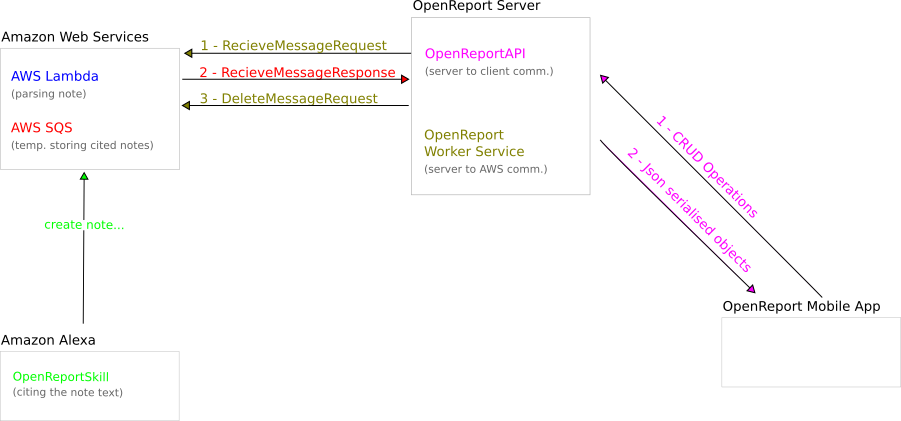
\includegraphics[width=11cm]{plan}
\end{center}
\caption{Visokonivojski načrt sistema}
\label{plan}
\end{figure}

\section{Uporabljene tehnologije in programska oprema}

\subsection{.NET}

.NET je razvojna platforma, razvita s strani Microsofta.
Obsega programske jezike, prevajalnike, orodja in knjižnice, ki omogočajo širok spekter primerov uporabnosti, hkrati pa se ohranja enovitost ozadne kode.

Tehnologije .NET ogrodja, ki sem jih uporabil v tej diplomski nalogi so:
\begin{itemize}
	\item .NET Core - odprtokodna platforma za razvoj spletnih storitev,
	\item Xamarin, ki je ogrodje za razvoj mobilnih aplikacij za najpogostejše mobilne operacijske sisteme (Android, iOS).
\end{itemize}

.NET sem izbral, saj je zelo dobro integriran z Amazonovim AWS API-jem in ker je dobro dokumentiran.

\subsection{Xamarin Forms}

Ogrodje Xamarin je odprtokodno orodje za razvoj mobilnih aplikacij, ki ga je razvil Microsoft. 
% Je nadgradnja ogrodja .NET.

Z ogrodjem Xamarin je mogoče pri deliti večino ozadne in ospredne kode med različnimi mobilnimi operacijskimi sistemi. 
Za ozadno kodo se uporablja .NET (C\#), za front-end pa se uporablja XAML (Extensible Application Markup Language).

Xamarin sem izbral, saj imam z njim že predhodne izkušnje.

// še kakšen razlog?

\subsection{Amazon Alexa}

Amazon Alexa je glasovni asistent, razvit s strani podjetja Amazon.
Za Amazon Alexo sem se odločil, saj ponuja enostavno možnost programiranja s ''Skill-i''.
Poleg tega je Alexo enostavno integrirati z drugimi Amazonovimi spletnimi storitvami, kot so AWS SQS.

\subsection{Alexa Skill}

Alexine osnovne funkcionalnosti lahko nadgradimo s programi, ki se jim reče ''Skill''.
Da lahko ustvarimo in objavimo Skill rabimo račun Amazon razvijalca (\textit{ang. Amazon Developer Account}).


''Skill'' sestavljajo:
\begin{itemize}
	\item Invocation - fraza, ki ''Skill'' zažene,
	\item Intent - fraze, ki jih Skill razpozna kot funkcije,
	\item Endpoint - omrežni vir, kjer se nahaja ozadna koda ''Skill-a''.
\end{itemize}

Ko Alexa zasliši Invocation ali katerega od Intentov, glasovni posnetek pošlje na Amazonov strežnik.
Ta s pomočjo glasovnega razpoznavnega modela prepozna ukaze in pošlje poseben zahtevek na Endpoint.
To je lahko druga Amazonova storitev (npr. AWS Lambda), storitev na Microsoftovem Azure strežniku ali naš lasten strežnik, dostopen preko javne domene.

Ko Endpoint obdela zahtevo, se odgovor pošlje nazaj na Amazonov strežnik v obliki znakovnega niza.
Ta podatek se nato pošlje nazaj na uporabnikovo Alexo, ki prejeti znakovni niz ''izgovori''.

\subsection{Amazon Web Services}

AWS je skupek oblačnih storitev, ki ga ponuja podjetje Amazon.
Ponuja integracijo s popularnimi programskimi jeziki in ogrodji, kot so Java, .NET, Python in Node.js preko AWS API storitve.
Pri tej diplomski nalogi sem se osredotočil na dva sistema iz skupka AWS.

\subsubsection{AWS SQS}

AWS SQS je sistem za pošiljanje tekstovnih sporočil med odjemalci preko Amazonovih strežnikov.
Za hranjenje sporočil je treba registrirati SQS Queue \textit{(slo. SQS vrsto)}. 
Ta je lahko neurejena vrsta, kjer prejeta sporočila niso nujno urejena po času ustvarjanja, lahko pa je tipa FIFO, pri kateri je zagotovljeno, da dobimo vsa sporočila v vrstnem redu, v katerem so bila poslana.
V sklopu te diplome sem uporabil vrsto FIFO.

To storitev bom uporabil za komunikacijo med Amazon Alexo in OpenReport strežnikom.

// ali še opišem SQS?

\subsubsection{AWS Lambda}

Ozadno kodo za Alexa Skill sem gostil na platformi AWS Lambda.
To je storitev za gostovanje dogodkovno vodene ozadne kode.
Za to platformo smo se odločili zaradi dobre integracije z Alexa Skill Kit-om in razvojnim orodjem Visual Studio.

// ali še opišem Lambdo?


\section{Strežnik}

Za uporabo centralnega strežnika smo se odločili, da lahko do hranjenih podatkov dostopamo iz različnih naprav preko enotnega vmesnika (API).
V našem primeru bosta s strežnikom komunicirala mobilna aplikacija in glasovni asistent.
Podatke bomo hranili v podatkovni bazi, ki jo streže SQL Server.

Baza hrani tabele Users (\textit{slo. Uporabniki}), Projects (\textit{slo. Projekti}) in Notes (\textit{slo. Zapiski}).
Vsak uporabnik lahko ima 0 ali mnogo projektov (opisov tehnološkega postopka).
Vsak projekt ima lahko 0 ali mnogo zapiskov (korakov).

// naredi sliko sheme baze

\noindent Strežnik ima naslednje naloge:
\begin{enumerate}
	\item komunikacija s podatkovno bazo,
	\item komunikacija z odjemalcem (mobilno aplikacijo),
	\item komunikacija z glasovnim asistentom (Amazon Alexa),
	\item ponujanje vmesnika, preko katerega lahko odjemalci delajo s podatki v bazi.
\end{enumerate}


\subsection{Implementacija API}

Komunikacija med strežnikom in odjemalci poteka preko HTTP po pristopu API.
Podatki se prenašajo v formatu JSON.
To metodo smo izbrali zaradi enostavnosti implementacije in možnosti širjenja v prihodnosti.

Glede na to, da lahko sistem uporablja več uporabnikov, sem se odločil implementirati sistema za avtentikacijo uporabnikov in avtorizacijo zahtev.
Avtentikacija z uporabniškim imenom in geslom omogoča preverjanje identitete.
Ko se vzpostavi zaupanje, se prijavljenemu uporabniku dodeli avtorizacijski žeton, iz katerega se da razbrati, za katerega uporabnika gre in katere pravice so mu dodeljene.

\subsubsection{Registracija in prijava}

Odjemalec mora poslati na API objekt razreda \textit{RegisterUserRequest}.
Odjemalec ga mora poslati na URL ''\texttt{/identity/register}''.

\noindent \texttt{RegisterUserRequest \{ \\
	string Email; \\
	string Password; \\
\} }

Ko strežnik prejme ta objekt, ga pošlje v avtentikacijsko storitev.
V tej storitvi preveri, ali uporabnik že obstaja.
Če obstaja, se zabeleži napaka in nadaljnja registracija prekine.
Če ta uporabnik ne obstaja, se polje \texttt{Password} zakriptira in se skupaj s poljem \texttt{Email} zapiše v bazo.
Uporabnik pa pri registraciji dobi tudi svoj unikaten identifikator \texttt{UserID}.

V kolikor se je v avtentikacijski storitvi dogodila kakršna koli napaka, se klientu vrne objekt razreda \texttt{AuthFailedResponse}

\noindent \texttt{AuthFailedResponse \{ \\
  IEnumerable<string> Errors; \\
\} }

\noindent V tem objektu se odjemalcu v zbirki pošljejo vse napake, ki jih je avtentikacijska storitev zabeležila pri neuspešni registraciji.  Če je bila registracija uspešna, se odjemalcu pošlje objekt razreda \texttt{AuthSuccessResponse}

\noindent \texttt{AuthSuccessResponse \{ \\
  string UserId; \\
  string Token; \\
\} }

\noindent V polje \texttt{Token} se zapiše avtorizacijski žeton.
Žeton je tipa JWT ali \textit{JSON Web Token}.
Sestavljajo ga e-mail uporabnika, uporabnikov unikatni identifikator \texttt{UserID}, čas zapada žetona in tip simetričnega kodiranja, uporabljenega za enkripcijo žetona.

Ta objekt se nato pošlje nazaj odjemalcu.
Odjemalec nato ta žeton doda glavi vseh svojih HTTP zahtevkov na OpenReport strežnik.
V nadaljnji komunikaciji, strežnik iz žetona razbere uporabnikov unikatni identifikator in ga uporabi pri poizvedbah po podatkovni bazi.

Prijava poteka podobno.
Uporabnik mora poslati na API objekt \textit{LoginUserRequest}.
URL, na katerega mora odjemalec poslati ta objekt, je \texttt{/identity/login}.

\noindent
\texttt{LoginUserRequest \{ \\
  string Email; \\
  string Password; \\
\} }

Ko strežnik prejme ta objekt, ga pošlje v avtentikacijsko storitev.
V tej storitvi preveri, ali uporabnik že obstaja.
Če ta uporabnik ne obstaja, ali pa je njegovo zakriptirano geslo v podatkovni bazi drugačno kot to, kar je v polju \texttt{Password}, se zabeležijo napake in prijava se prekine.
Odjemalec prejme objekt razreda \texttt{AuthFailedResponse}.

Če uporabnik obstaja in se njegovo zakriptirano geslo iz polja \texttt{Password} ujema z geslom v podatkovni bazi, je avtentikacija uspešna.
Odjemalec prejme objekt razreda \texttt{AuthFailedResponse}.

V primeru uspešne avtentikacije se avtorizacijski žeton \texttt{Token} generira in pošlje enako kot pri registraciji.

\subsubsection{Operacije z delavniškimi dnevniki}

Vsak uporabnik lahko ima nič ali več delavniških dnevnikov.

Vse operacije nad uporabnikovim delavniškim dnevnikom morajo biti avtorizirane.
V kolikor niso, bo API vedno javil napako \texttt{Bad Request: Not Authorised}.

Pri ustvarjanju novega opisa tehnološkega postopka (v nadaljevanju poglavja \textit{projekta}) mora uporabnik podati naslov, kratek opis projekta in seznam možnih nevarnosti.

To odjemalec zapiše v objekt razreda \texttt{CreateProjectRequest}.

\noindent \texttt{CreateProjectRequest \{ \\
string Title; \\ 
string Description; \\
string Dangers; \\
\} }

\noindent Ta objekt se nato pošlje preko POST metode na strežnik na naslov \texttt{/projects/create}.
Storitev za operacije nad projekti nato kreira nov objekt razreda \texttt{Project} s podatki iz prejete zahteve.
V primeru, da je zahteva ustrezno formulirana in avtorizirana, se projekt zapiše v podatkovno bazo.
Odjemalcu se kot odgovor pošlje kopija tega projekta.

\noindent Razred \texttt{Project} izgleda tako:

\noindent \texttt{Project \{ \\
int Id; // unikatni identifikator \\
string Title; \\
string Description; \\
string Dangers; \\
IEnumerable<Note> Notes; // seznam korakov \\
... \\
\}
}


Do kateregakoli svojega projekta lahko odjemalec v nadaljnji komunikaciji dostopa tako, da pošlje GET zahtevek na URL \texttt{/projects/\{id\}}.
Polje \texttt{id} mora v tem primeru biti unikatni identifikator projekta.

Za izbris projekta mora uporabnik poslati DELETE zahtevo na URL \texttt{/projects/\{id\}}.
Če zahteva ni avtorizirana z ustreznim žetonom, se projekt ne izbriše.

\subsubsection{Operacije nad koraki opisa tehnološkega postopka}

Vsak projekt ima lahko nič ali več korakov.
Vsak korak ima naslov, opis in predvideno trajanje.

Korak je lahko izključno tekstovni, lahko pa ima tudi pripadajočo sliko.

Da ustvarimo tekstovni korak moramo poslati objekt razreda \texttt{Note} preko POST metode na URL \texttt{/projects/\{id\}/addnote}.
Polje \texttt{id} mora biti unikatni identifikator projekta, katermu želimo dodati korak.

\noindent Razred \texttt{Note} izgleda tako.

\noindent \texttt{Note \{ \\
...\\ 
string Title; \\
string Text; \\
int Hours; \\
int Minutes; \\
int Seconds; \\
...\\ 
\} }

Strežnik najprej preveri, če je pošiljatelj poslal avtorizirano zahtevo.
Iz avtorizacijskega žetona strežnik razbere uporabnikov \texttt{UserID}. 
Če je projekt z identifikatorjem \texttt{id} res v lasti uporabnika z identifikatorjem \texttt{UserID}, se bo korak dodal v zbirko korakov tega projekta.

Če želimo ustvariti slikovni korak, moramo poslati objekt razreda \textit{AddImageRequest} na URL \texttt{/projects/\{id\}/addimage}.

\noindent \texttt{AddImageRequest \{ \\
Note note; \\
string ImageString;  \\
\} }

V tem razredu predstavlja polje \texttt{ImageString} pripadajočo fotografijo, zakodirano v znakovni niz.
Za kodirni algoritem sem uporabil Base64.

Za hranjenje tekstovnih in slikovnih korakov sem zaradi preprostosti implementacije uporabil isti razred \texttt{Note}.
Tekstovni in slikovni korak se ločita v vrednosti boolean zastavice \texttt{IsImage}.
Tekstovni korak ima to zastavico nastavljeno na vrednost \texttt{false}, slikovni pa \texttt{true}.

\noindent \texttt{Note \{ \\
\underline{bool IsImage;}  \\
string Title; \\
string Text; \\
int Hours; \\
int Minutes; \\
int Seconds; \\
\underline{string Url;} // Lokacija slike na klientu \\
\underline{string ServerUrl;} // Lokacija slike na strežniku \\
... \\
\}
}

Poljema \texttt{Url} in \texttt{ServerUrl} se dodeli vrednost samo pri slikovnih korakih.
Ko se na klientu zajame fotografija, klient nastavi vrednost polja \texttt{Url} na lokacijo ustvarjene fotografije v datotečnem sistemu.

Polje \texttt{ServerUrl} se nastavi šele na strežniku.
Ko strežnik prejme zahtevo za kreiranje slikovnega koraka, se korak \texttt{Note} prebere iz objekta \texttt{AddImageRequest} in zapiše v podatkovno bazo.
Nato se \texttt{ImageString} dekodira in hrani na strežniku.
Ko se fotografija uspešno zapiše v datotečni sistem, se v polje \texttt{ServerUrl} zapiše lokacija pravkar ustvarjene datoteke na strežniku in spremembe se hranijo v podatkovni bazi.

\subsubsection{Urejanje in brisanje in korakov v projektu}

Da se korak v projektu izbriše, moramo poslati avtorizirano zahtevo na URL \texttt{/projects/\{pid\}/delete/\{nid\}}.
V tem primeru je polje \texttt{pid} unikatni identifikator projekta, v katerem se nahaja korak, \texttt{nid} pa unikatni identifikator objekta \texttt{Note}, ki ga želimo izbrisati.
V kolikor ima ta objekt \texttt{Note} postavljeno zastavico \texttt{IsImage} na \texttt{true}, se poleg zapisa v bazi izbriše tudi pripadajoča slikovna datoteka.

Pri posodabljanju (urejanju) korakov, moramo poslati avtorizirano zahtevo na URL \texttt{/projects/\{pid\}/update/\{nid\}}.
Telo zahteve mora vsebovati objekt razreda \texttt{Note}.

// heyhey kaj pa slika?

\subsubsection{Spreminjanje vrstnega reda korakov v projektu}

Položaj koraka \texttt{Note} v projektu lahko razberemo iz atributa \texttt{Position}.
Prvi korak ima \texttt{Position} 0, drugi 1, itd.

\noindent \texttt{Note \{ \\
int Id; \\
\underline{int Position;} \\
bool IsImage;  \\
string Title; \\
string Text; \\
int Hours; \\
int Minutes; \\
int Seconds; \\
string Url; \\
string ServerUrl; \\
\}
}

Pri dodajanju korakov v projekt se obstoječe korake projekta razvrsti po vrednosti polja \texttt{Position}.
Vzamemo največjo vrednost tega polja in ji prištejemo 1.
Nato to vrednost priredimo polju \texttt{Position} novo kreiranega koraka.

Ko želimo spremeniti pozicijo koraka v projektu, moramo poslati zahtevo PUT na URL \texttt{/projects/\{pid\}/\{nid\}/\{positions\}}.

V tem primeru je polje \texttt{pid} unikatni identifikator projekta, v katerem se nahaja korak, \texttt{nid} unikatni identifikator koraka \texttt{Note}, in \texttt{Positions} število mest za kolikor ga želimo prestaviti.
To število je lahko pozitivno ali negativno celo število.
Negativna vrednost prestavi korak proti začetku seznama, pozitivna pa proti koncu.

\subsubsection{Izvoz projektov}

Projekt lahko izvozimo v dva formata, v tekstovno datoteko in HTML dokument.

To naredimo tako, da pošljemo avtorizirani GET zahtevi na URL-ja \texttt{/projects/\{id\}/export/text} ali \texttt{/projects/\{id\}/export/html}.

Pri izvozu v tekstovno datoteko storitev za upravljanje projektov na strežniku ustvari novo tekstovno datoteko.
Najprej vanjo vpiše naslov in opis projekta ter možne nevarnosti pri delu.
Nato uredi korake po vrednosti stolpca \texttt{Position} in enega za drugim zapiše v datoteko.
Če je korak slikovni, se zapiše tudi lokacija pripadajoče fotografije.

Pri izvozu v HTML dokument se naslov zapiše kot HTML naslov H1, opis kot naslov H2, in koraki kot HTML odstavki.
V HTML dokumentu lahko prikažemo poleg slikovnih korakov tudi slike same.

// slika exportanega 

Lokacija izvožene datoteke se nahaja v polju \texttt{FolderLocation} v razredu \texttt{Project}.
Privzeta lokacija, ki se nastavi ob kreiranju projekta je 
\\''\texttt{C:/users/USER/Public Documents/OpenReport}''.

\noindent \texttt{Project \{ \\
int Id; \\
string Title; \\
string Description; \\
string Dangers; \\
\underline{string FolderLocation;} // lokacija fotografij in izvoženih datotek \\
IEnumerable<Note> Notes; \\
... \\
\}
}

\subsection{Komunikacija strežnika z glasovnim asistentom}

Strežnik z glasovnim asistentom Amazon Alexa komunicira preko storitve AWS SQS.
Glasovni asistent od uporabnika prejme glasovni ukaz.
Na podlagi tega ukaza lahko glasovni asistent na SQS vrsto odloži tri različna tekstovna sporočila:
\begin{itemize}
	\item "addnote",
	\item "addimage",
	\item "\{narekovano besedilo\}",
\end{itemize}

// ali tukaj opišem kaj delajo??

\subsubsection{Utemeljitev uporabe SQS}
Za hranjenje sporočil v storitvi SQS smo se odločili po primerjavi z dvema alternativnima pristopoma.
Prvi je bil odpiranje omrežne vtičnice (ang. Web Socket).
Ta bi prinesla učinkovitejši prenos podatkov, implementacija pa bi bila težja.
Druga alternativa pa je bila direktna komunikacija Amazon Alexe in našega strežnika preko REST API zahtevkov, ki se prenašajo po protokolu HTTP.
Ta alternativa bi bila implementacijsko preprostejša kot uporaba SQS.
Problem te alternative bi bil, da bi bilo treba javno odpreti API dostopne točke, ki jih lahko asistent uporablja, ali implementirati nove metode za avtentikacijo in avtorizacijo zahtevkov iz glasovnega asistenta.

\subsubsection{Zahtevanje in izpust glasovnega asistenta}

V sklopu našega projekta bomo na enem OpenReport strežniku uporabljali samo enega glasovnega asistenta.
Tega asistenta lahko uporabnik ''zahteva'' za lastno uporabo in ga po uporabi ''izpusti''.
Ali ima določen uporabnik nase vezanega asistenta, vidimo po vrednosti zastavice \texttt{UsesVoiceAssistant} v njegovem objektu razreda \texttt{User}.

Ko uporabnik odpre katerega od svojih projektov, se unikatni identifikator tega projekta nastavi v polje \texttt{LastOpenedProjectId} v njegovem objektu razreda \texttt{User}.

Zahtevki, ki jih strežnik prejme od glasovnega asistenta, se navezujejo na ta projekt.

\noindent \texttt{User : IdentityUser \{ \\
string Id; \\
string Email; \\
string Password; \\
IEnumerable<Project> Projects; \\
... \\
\underline{int LastUsedProjectId;} \\
\underline{bool UsesVoiceAssistant;} \\
\}}

\subsubsection{Delovanje}

Na strežniku OpenReport teče storitev za komunikacijo z glasovnim asistentom.
Ta storitev vsakih deset sekund na SQS pošlje zahtevek \texttt{RecieveMessageRequest}.
\noindent\texttt{RecieveMessageRequest \{ \\
AttributeName \\ % // obsežnost filtriranja podatkov v sporočilih \\
MaxNumberOfMessages \\ % // koliko sporočil naenkrat lahko prejmemo \\
QueueUrl \\ %// URL SQS vrste\\ % \\
WaitTimeSeconds \\ %// kako dolgo SQS počaka na morebitno prihajajoče sporočilo \\
... \\
\} 
}

AWS SQS kot odgovor vrne objekt tipa \texttt{RecieveMessageResponse}.

\noindent\texttt{RecieveMessageResponse \{ \\
IEnumerable<Message> Messages;\\
... \\
\} }

V tem odgovoru se nahaja seznam sporočil, ki čakajo na sprejem iz SQS vrste.
V kolikor je v odgovoru vsaj eno sporočilo, pregledamo telo vseh sporočil. 

Ko sporočila sprejmemo, jih moramo izbrisati iz SQS vrste.
Če jih sproti ne izbrišemo, iz FIFO vrste ne moremo brati najnovejših sporočil, ampak le 5 najstarejših.

Sporočila izbrišemo iz vrste preko zahtevka \texttt{DeleteMessageRequest}.
AWS SQS storitev v odgovor vrne \texttt{DeleteMessageResponse}, a v tej diplomski nalogi tega odgovora ne uporabljamo naprej.

Zahtevki, ki jih prejmemo od glasovnega asistenta v projektu, ki ga je uporabnik z glasovnim asistentom nazadnje odprl, nastavijo vrednosti treh boolean zastavic v objektu razreda \texttt{Project}.
\begin{itemize}
	\item Zahtevek ''\texttt{addnote}'' nastavi zastavico ''\texttt{NoteRequest}'' na \texttt{true},
	\item zahtevek ''\texttt{addimage}'' nastavi zastavico ''\texttt{ImageRequest}'' na \texttt{true},
	\item zahtevek ''\texttt{\{narekovano besedilo\}}'' nastavi zastavico ''\texttt{AlexaNoteRequest}'' na \texttt{true} in prejeto besedilo doda projektu kot korak.
\end{itemize}

\noindent \texttt{Project \{ \\
int Id; \\
string Title; \\
string Description; \\
string Dangers; \\
string FolderLocation; \\
IEnumerable<Note> Notes; \\
\underline{bool NoteRequest;} \\
\underline{bool ImageRequest;} \\
\underline{bool AlexaNoteRequest;} \\
\}
}



Če je vsebina prejetega sporočila enaka \texttt{addnote}, storitev preveri, kateri uporabnik ima trenutno nase vezanega glasovnega asistenta.
Nato v projektu, katerega je nazadnje odprl nastavi vrednost zastavice \texttt{NoteRequest} na \texttt{true}.


Če je vsebina enaka ''\texttt{addimage}'', storitev preveri, kateri uporabnik ima trenutno nase vezanega glasovnega asistenta.
Nato v projektu, katerega je nazadnje odprl nastavi vrednost zastavice \texttt{ImageRequest} na \texttt{true}.

Če vsebina prejetega sporočila ni enaka ''\texttt{addimage}'' ali ''\texttt{addnote}'', pomeni, da je prejeto sporočilo dobesedno narekovan korak.
Kot prej, storitev preveri, kateri uporabnik ima nase vezanega glasovnega asistenta.
Nato v projektu, katerega je nazadnje odprl nastavi vrednost zastavice \texttt{AlexaNoteRequest} na \texttt{true}.
Poleg tega ustvari nov objekt razreda \texttt{Note}, ki ima naslov ''Voice note'', vsebina pa je telo prejetega sporočila.
Nov objekt se nato vstavi v najden projekt.

% \subsubsection{Registracija na AWS SQS}
% 
% // kaj rabimo da registriramo in uporabimo SQS
% 
% // mogoce prestavim za skill?





\section{Implementacija ,,Alexa Skilla''}

// narekovaje bom popravil, ko bo vsebinsko ok

Alexa Skill bomo uporabili za glasovno upravljanje aplikacije.
Glavni namen Alexa Skilla v sklopu sistema OpenReport bo dodajanje korakov v opis tehnološkega postopka.

\noindent Natančneje, Skill bo uporabniku omogočal:
\begin{itemize}
	\item dodajanje tekstovnega koraka,
	\item odpiranje kamere in dodajanje slikovnega koraka in
	\item dobesedno narekovanje besedila tekstovnega koraka.
\end{itemize}

Ko bo Alexa zaslišala ukaz za zagon skilla (ang. Invocation), se bo Skill začel izvajati.
Ta fraza se glasi ''\textit{make a report note}''.

Vsak nadaljnji ukaz, ki ga bo uporabnik izrekel, preden se Skill preneha izvajati, se bo primerjal s frazami za zagon podprogramov Skilla.
Te fraze se imenujejo ''namere'' (ang. Intent).
V našem skillu bomo imeli tri glavne namere:

\begin{itemize}
	\item \texttt{TakeNoteIntent},
	\item \texttt{OpenTextNoteFormIntent},
	\item \texttt{OpenImageNoteFormIntent}.
\end{itemize}

// slike intentov v alexa developer console

\texttt{TakeNoteIntent} se bo zagnal, ko bo po invokacijski frazi uporabnik izrekel ''\texttt{take note \{besedilo\}}'' ali ''\texttt{note \{besedilo\}}''.
\texttt{\{besedilo\}} je tekstovna spremenljivka, v katero Skill hrani razpoznano tekstovno vsebino koraka.
V primeru, da uporabnik izreče ''\textit{note unscrew the backplate}'', bo vrednost spremenljivke \texttt{\{besedilo\}} ''unscrew the backplate''.

Ta Intent bo v ozadni kodi Skill-a zagnal funkcijo, ki bo ustvarila novo SQS sporočilo.
V telo tega sporočila bo funkcija vstavila vrednost spremenljivke \texttt{\{besedilo\}} in ga poslala v SQS vrsto.
Skill zatem vrne uporabniku odgovor ''Noted!'' in se preneha izvajati.

\texttt{OpenTextNoteFormIntent} se bo zagnal, ko bo po invokacijski frazi uporabnik izrekel ''\texttt{create a text note}''.

Ta Intent bo v ozadni kodi Skill-a zagnal funkcijo, ki bo ustvarila novo SQS sporočilo.
V telo tega sporočila bo funkcija vstavila vrednost ''\texttt{addnote}'' in ga poslala v SQS vrsto.
Skill zatem vrne uporabniku odgovor ''Opening the form!'' in se preneha izvajati.

\texttt{OpenImageNoteFormIntent} se bo zagnal, ko bo po invokacijski frazi uporabnik izrekel ''\texttt{take a picture}''.

Ta Intent bo v ozadni kodi Skill-a zagnal funkcijo, ki bo ustvarila novo SQS sporočilo.
V telo tega sporočila bo funkcija vstavila vrednost ''\texttt{addimage}'' in ga poslala v SQS vrsto.
Skill zatem vrne uporabniku odgovor ''Launching camera!'' in se preneha izvajati.


\subsection{Izvajanje ''Skill-a'' po korakih}

Alexa Skill se bo začel izvajati, ko uporabnik izreče definirano invokacijsko frazo.
Alexa posnet govorni ukaz pošlje na Amazonov Alexa Server.
Tam se s pomočjo NLU razpoznavnega modela poskusi pretvoriti v znakovni niz.
Ta znakovni niz se primerja z vsemi definiranimi invokacijskimi frazami za Skill-e, ki so vezani na naš Amazon račun.

Če Alexa Server uporabnikov glasovni ukaz razpozna kot ,,make a report note'', se začne izvajati OpenReportAlexaSkill.
V ozadno kodo Skill-a (ang. Endpoint) se pošlje zahteva tipa \texttt{LaunchRequest}.
Endpoint nastavimo v Alexa Developer Console.
Lahko je AWS Lambda funkcija, lahko pa je naš lasten strežnik, dostopen preko javne domene.
Endpoint je v našem primeru gostovan na storitvi AWS Lambda.
Ob prejetju \texttt{LaunchRequest} Endpoint našega Skilla vrne vprašanje ''What now?''.


Naslednji glasovni ukaz se primerja s frazami za namere (ang. Intent).
Če se ukaz ujema z frazami, ki zaženejo katerega od Intent-ov TakeNoteIntent, OpenTextNoteFormIntent ali OpenImageNoteFormIntent, se na Endpoint pošlje zahteva tipa \texttt{IntentRequest}.

Iz prejetega \texttt{IntentRequest}-a nato dobimo ime Intent-a.
Na podlagi imena prejetega Intent-a ločimo, ali gre za TakeNoteIntent, OpenTextNoteFormIntent ali OpenImageNoteFormIntent in zaženemo funkcije, opisane v prejšnjem poglavju.


\begin{figure}[H]
\begin{center}
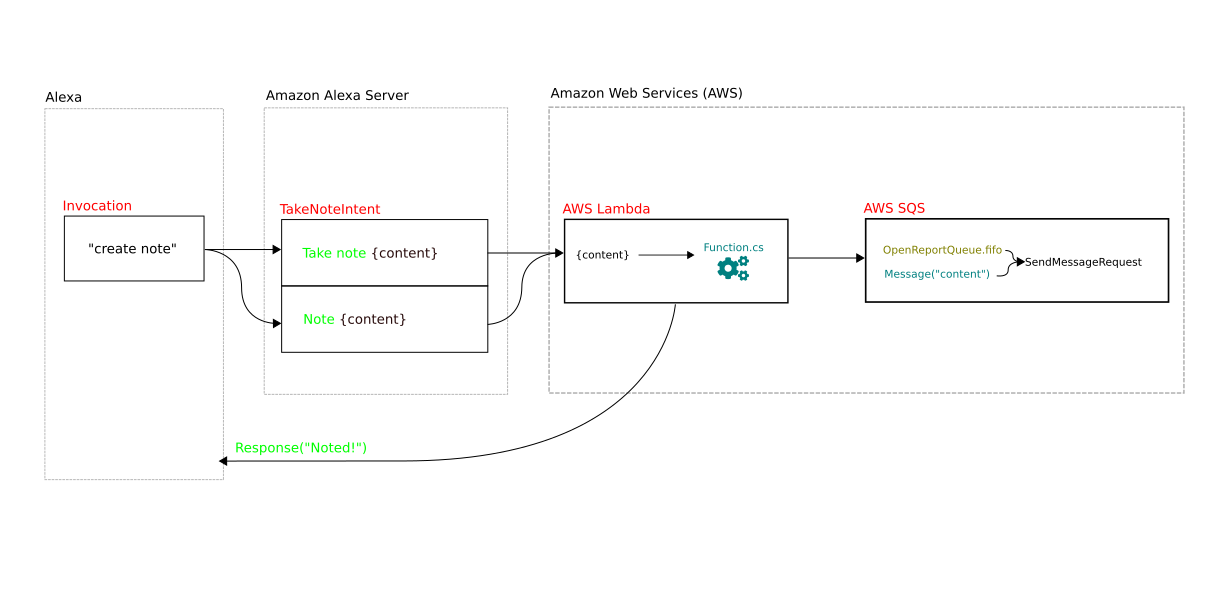
\includegraphics[width=11cm]{skill}
\end{center}
\caption{Načrt Alexa Skilla}
\label{skill}
\end{figure}

\section{Implementacija mobilne aplikacije}

Mobilna aplikacija bo služila kot osnoven način za interakcijo s strežnikom.
Do strežnika bo dostopala preko API vmesnika.
Zahtevki se bodo prenašali preko HTTP protokola.

Mobilno aplikacijo sem se odločil razviti s tehnologijo Xamarin.Forms.
Razlogi za to so predvsem dobro poznavanje tehnologije in enostavna integracija z ostalimi tehnologijami iz .NET sklopa.


\subsection{Pristop}
Pristop razvoja aplikacije, ki smo ga uporabili za programiranje aplikacije, se imenuje Model View View-Model (v nadaljevanju MVVM).
Pri tem pristopu aplikacijo razdelimo na tri dele.

\textbf{Model} je del, kjer definiramo elemente naše ''poslovne logike'' (opis tehnološkega postopka, korak, uporabnik,...).

\textbf{View} je uporabniški vmesnik, ki ga vidi uporabnik.

\textbf{ViewModel} pa se uporablja, da se poveže funkcije uporabniškega vmesnika in modela (''poslovne logike'') ter po potrebi preoblikuje podatke.

Rezultat upoštevanja tega pristopa je čista koda, ki se ne prepleta.
Model vsebuje le abstrakcijo naših podatkov in poslovno logiko.
Ti podatki se v ViewModelu pretvorijo v obliko, ki bo prikazana uporabniku.
View pa vsebuje izključno grafične elemente.

// slika mvvm

\subsection{Povezava na strežnik, prijava in registracija uporabnika}

Ob zagonu mobilne aplikacije, uporabnika pričaka stran za povezavo na OpenReport strežnik.
V tekstovno polje mora vpisati URL ali IP strežnika.
Ta naslov bomo v nadaljevanju podpoglavja označevali z \texttt{naslovstrežnika}.

// slika povezavne strani

Ko uporabnik klikne gumb ''Connect'', se preveri, ali je naslov pravilnem formuliran.
Če je, storitev za komunikacijo s strežnikom pošlje neavtorizirano zahtevo na ''\texttt{naslovstrežnika}/connect''. 
Če je na tem naslovu res OpenReport strežnik, se kot odgovor odjemalcu pošlje boolean vrednost \texttt{true}.

Storitev za komunikacijo s strežnikom si nato hrani vrednost \texttt{naslovstrežnika} kot predpono vseh nadaljnjih zahtevkov.

Ob neuspešnem poskusu povezave se uporabniku na strani prikaže opis napake.
Če je poskus uspešen, se stran za povezavo na strežnik zapre.

Prikaže se stran za prijavo.
Na tej strani uporabnik vpiše svoje uporabniško ime ali geslo, lahko pa odpre stran za registracijo računa.

Poskus prijave poteka tako, avtentikacijska storitev uporabniško ime in geslo iz prijavne strani zapiše v objekt razreda \texttt{LoginUserRequest}.

\noindent \texttt{LoginUserRequest \{ \\
	Email; \\
	Password; \\
\} }

Nato se ta objekt pošlje na strežnik na URL \texttt{/identity/login} preko POST metode.
Strežnik ob uspešni avtentikaciji vrne objekt razreda \texttt{AuthSuccessResponse}.
Iz tega objekta uporabnik prebere svoj avtorizacijski žeton.
Ta žeton hrani avtentikacijska storitev.
Pri nadaljnjih poizvedbah komunikacijska storitev ta žeton doda v glavo HTTP zahtevkov.

Če je avtentikacija neuspešna, strežnik vrne objekt razreda \texttt{AuthFailedResponse}, v katerem je podan opis napake.
Ta opis napake se nato uporabniku izpiše na prijavni strani.

Stran za registracijo je podobna strani za prijavo, le da ima dve vnosni polji za vpis gesla.
Drugo vnosno polje je preventivni ukrep, da se uporabnik ne registrira z napačno vtipkanim geslom.

Registracijski zahtevek se pošlje na strežnik na URL \texttt{/identity/register}.
Zahtevek je objekt razreda \texttt{RegisterUserRequest}.

\noindent \texttt{RegisterUserRequest \{ \\
	Email; \\
	Password; \\
\} }

// dodaj sliko registracijske strani in prijavne strani

\subsection{Ustvarjanje, brisanje in odpiranje projektov}

\subsection{Zahtevanje in izpust glasovnega asistenta}

\subsection{Operacije znotraj projekta}


% koga briga
% \subsection{Uvoz knjižnic in zunanjih virov v projekt}
% Po dizajnu sem se lotil programiranja.
% Najprej sem ustvaril prazen Xamarin projekt tipa Shell.
% Najprej sem želel uvoziti funkcionalnosti, ki bi mi v prihodnjih fazah olajšale delo.
% Prva taka stvar je bila uvoz razširitev Fody.
% To je orodje, ki med prevajanjem MVVM aplikacije določene odseke C\# kode "vstavi" v preveden assembly.
% S tem se ohrani ista funkcionalnost z veliko manj boilerplate kode.
% 
% // slika fody
% 
% Naslednja takšna funkcionalnost je bila uvoz fontov.
% Za ikone nisem uporabil SVG ali PNG zbirk, ampak sem uporabil popularen font FontAwesome, ki ga nekoliko enostavneje uporabiti in uvoziti.
% 
% V projektu OpenReportShell.Android sem v Assets mapo dodal podmapo fonts.
% V tej mapi se nahaja datoteka s FontAwesome Solid fontom.
% 
% Ta font sem uporabil tako, da sem v osnovnem projektu dodal Resource v datoteki App.xaml.
% 
% // slika resource

\subsection{Povezava na strežnik in razred Startup.cs}

// razlozi kot normalen človek

Za povezavo na strežnik sem želel v projektu imeti eno instanco statičnega razreda.
Ta razred (OpenReportCloudCommunicationService) vsebuje metode, namenjene komunikaciji z API-jem.

Registriral sem ga po metodi DependencyInjection.
To sem dosegel tako, da sem v projekt dodal razred Startup.cs.
V tem razredu sem registriral razred ServiceProvider, s katerim bom lahko dostopal do registriranih razredov drugod po aplikaciji.

V ServiceProvider sem dodal dva razreda.
Prvi je HttpClient, ki sem ga uporabil za pošiljanje HTTP sporočil na strežnik, drugi pa je OpenReportServerCommunicationService, ki je bil uporabljen za formiranje HTTP sporočil.

// slika ConfigureServices

// slika OpenReportServerCommunicationService


\subsection{DashboardPage}

// koga briga, spremeni 

Na strani DashboardPage se uporabniku prikaže seznam odprtih projektov.
Ko uporabnik klikne na željeni projekt, ga preusmeri na stran ProjectPage, kjer ga lahko ureja.
Če nanj pridrži, se mu pokažejo dodatne opcije, kot so izbris in ahriviranje.

// slika DashboardPage

\subsection{ProjectPage}

Najpomembnejši del aplikacije je urejanje zapiskov.
To lahko uporabnik dela, 



\section{Evalvacija funkcionalnosti}

\chapter{Možnosti nadaljnega razvoja}
\chapter{Zaključek}

% \section{Formati slik}
% 
% Bitne slike, vektorske slike, kakršnekoli slike, z \LaTeX{}om lahko vključimo vse.
% Slika~\ref{pic1} je v {\tt .pdf} formatu.
% \begin{figure}[h]
% \begin{center}
% 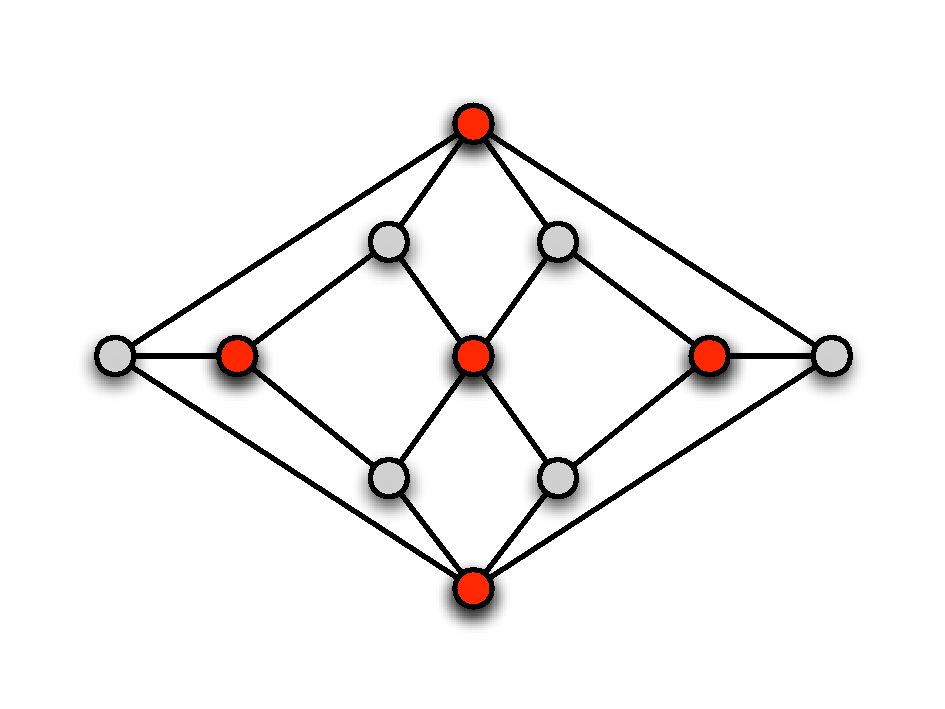
\includegraphics[width=0.6\textwidth]{pic1.pdf}
% \end{center}
% \caption{Herschelov graf, vektorska grafika.}
% \label{pic1}
% \end{figure}
% Pa res lahko vključimo slike katerihkoli formatov? 
% Žal ne. 
% Programski paket \LaTeX\ lahko uporabljamo v več dialektih. 
% Ukaz {\tt latex} ne mara vključenih slik v formatu Portable Document Format {\tt .pdf}, ukaz {\tt pdflatex} pa ne prebavi slik v Encapsulated Postscript Formatu {\tt .eps}.
% Strnjeno je vključevanje različnih vrst slikovnih datotek prikazano v tabeli~\ref{tbl:1}.


\newpage %dodaj po potrebi, da bo številka strani za Literaturo v Kazalu pravilna!
\ \\
\clearpage
\addcontentsline{toc}{chapter}{Literatura}

%\printbibliography

\end{document}
